\documentclass[runningheads]{llncs}

% ---------------------------------------------------------------
% Include basic ECCV package
 
% TODO REVIEW: Insert your submission number below by replacing '*****'
% TODO FINAL: Comment out the following line for the camera-ready version
%\usepackage[review,year=2026,ID=6131]{eccv}
% TODO FINAL: Un-comment the following line for the camera-ready version
\usepackage{eccv}

% OPTIONAL: Un-comment the following line for a version which is easier to read
% on small portrait-orientation screens (e.g., mobile phones, or beside other windows)
%\usepackage[mobile]{eccv}


% ---------------------------------------------------------------
% Other packages

% Commonly used abbreviations (\eg, \ie, \etc, \cf, \etal, etc.)
\usepackage{eccvabbrv}

% Include other packages here, before hyperref.
\usepackage{graphicx}
\usepackage{amssymb}
\usepackage{booktabs}
\usepackage{wrapfig}
\usepackage{makecell} % 必须加载这个宏包才能使用 \makecell 命令
\usepackage{array} 
\usepackage{adjustbox}

% The "axessiblity" package can be found at: https://ctan.org/pkg/axessibility?lang=en
\usepackage[accsupp]{axessibility}  % Improves PDF readability for those with disabilities.


% ---------------------------------------------------------------
% Hyperref package

% It is strongly recommended to use hyperref, especially for the review version.
% Please disable hyperref *only* if you encounter grave issues.
% hyperref with option pagebackref eases the reviewers' job, but should be disabled for the final version.
%
% If you comment hyperref and then uncomment it, you should delete
% main.aux before re-running LaTeX.
% (Or just hit 'q' on the first LaTeX run, let it finish, and you
%  should be clear).

% TODO FINAL: Comment out the following line for the camera-ready version
%\usepackage[pagebackref,breaklinks,colorlinks,citecolor=eccvblue]{hyperref}
% TODO FINAL: Un-comment the following line for the camera-ready version
\usepackage{hyperref}

% Support for ORCID icon
\usepackage{orcidlink}

\newcommand{\fixme}[1]{{\textcolor{cyan}{[wenhan: #1]}}}
\newcommand{\hq}[1]{{\textcolor{red}{[Huaqiu: #1]}}}

\begin{document}

% ---------------------------------------------------------------
% TODO REVIEW: Replace with your title
%\title{EchoStyle: Towards authentic, expandable, and high-quality video style transfer} 
\title{EchoStyle: Unlocking High-Fidelity Video Stylization with Reverse Data Synthesis}

% TODO REVIEW: 如果标题太长，可以在这里设置运行头标题（通常单行能放下就不需要改，或者简写）
\titlerunning{EchoStyle: Video Stylization with Reverse Data Synthesis}

% TODO FINAL: 修复了非法空格、反斜杠，并为 \dagger 加上了数学环境
\author{Huaqiu Li$^{*}\inst{1,2} \and
Jiahao Wang$^{*}\inst{2,3} \and
Sijia Cai$^{\dagger}\inst{2} \and 
Hualian Sheng\inst{2} \and
Bing Deng\inst{2} \and
Jieping Ye\inst{2} \and
Wenhan Luo$^{\dagger}\inst{1}
}

% TODO FINAL: 规范填入运行头作者简写（姓氏保留，名字缩写；多于两位作者用 et al.）
\authorrunning{H. Li et al.}

% TODO FINAL: 修复了机构列表中的非法字符，规范了邮箱和链接的排版
\institute{The Hong Kong University of Science and Technology \and
Alibaba Group \and
Xi'an Jiaotong University\\ % 修复了 Xian 的拼写（应为 Xi'an）
\url{https://echostyle2026.github.io/} \\
\email{lihuaqiu2025@gmail.com}}

\maketitle

% 展示多样性；short；long；加一些case展示一下
\begin{figure}[htbp] % h:当前位置, t:顶部, b:底部, p:单独一页
    \centering % 使图像居中
    \includegraphics[width=\textwidth]{pdf/teaser.pdf} 
    % width=0.8\textwidth 表示图像宽度为正文宽度的 80%
    % image-file-name 是文件名（不需要加 .jpg 或 .png 后缀）
    %\caption{EchoStyle provides an stable solution for text-driven video stylization across diverse artistic domains while ensuring robust temporal and structural consistency.}
    \caption{EchoStyle provides a robust framework for video stylization across expansive artistic domains. By maintaining stringent temporal and motion coherence, it delivers visually compelling results that remain consistent even during long-video inference.}
    %\vspace{-5mm}
    \label{fig:teaser} % 用于文中引用的标签
\end{figure}
\footnotetext{*: Co-first Author.}
\footnotetext{$\dagger$: Corresponding Author.}

\begin{abstract}
  % 在图片风格化已经发展成熟的今天，视频风格化仍是智能创作中一个亟需解决的问题。由于现实中缺乏公开可用的成对视频数据，以往的方法或者基于图像训练，或者基于非端到端处理，并不能解决风格丢失，画质低以及大motion的情形。在本论文中，我们首次提出了authentic, scalable, and high-quality的视频风格迁移方法“echostyle”，通过提出可复用至多种风格的视频配对数据pipeline，提供高质量训练数据。同时，我们设计了基于wan的v2v架构，通过lora高效微调以及文本提示来完成风格编辑。之外，我们引入时序自回归token，将生成拓展至分钟级。echostyle在多种风格转换，尤其是动漫风格中取得了令人惊艳的效果，与商业模型相比，仍然取得sota。我们承诺会开源相关权重与代码。
  %过往的方法受限于成对的数据集获取，多采用基于图像的数据集或非端到端训练，导致伪影，闪烁，卡顿等低质问题。同时，缺乏合适的，expandaple的video2video框架支持长视频的转绘。
While image stylization has been studied extensively, video stylization remains a critical and largely unsolved challenge in the field of intelligent content creation. Existing methods, usually utilizing a reference image as the style prior, suffer from content leakage, data scarcity and limited adaptability to long videos, leading to suboptimal results with severe style drift and motion distortion. For these issues, we present EchoStyle, a scalable text-driven framework to achieve high-quality stylization of videos with arbitrary lengths. To start with, we construct a video-to-video architecture to appropriately re-fuse the video content and the text style. To address data scarcity, we pioneer an automatic reverse-synthesis pipeline to establish V-Style20k, a large-scale stylization dataset of 20k high-quality video pairs. To facilitate long video stylization, we devise an init-follow-mode mechanism along with a sliding-window inference strategy. Extensive experiments demonstrate EchoStyle's excellent performance across a wide range of artistic styles, even comparable to leading closed-source solutions. All the codes, model weights and dataset will be open-sourced.

% pioneer an automatic paired video data generation pipeline that is reusable across any styles, providing a source of high-quality paired video data.
%   Building upon the Wan2.2-I2V foundation, we propose a streamlined yet effective Video-to-Video architecture, introducing a multi-visual conditional control module to integrate diverse inputs, which is adaptable to both short- and long-duration video stylization.
%   Furthermore, we incorporate a temporally recurrent multi-frame token mechanism to extend the inference to minute-long videos. 
%   %As shown in Fig.~\ref{fig:teaser}, 
%   EchoStyle demonstrates excellent performance across a wide range of artistic styles, delivering particularly stunning results in anime stylization, even achieving comparable results with leading closed-source solutions. The code, model weight and dataset will be open-soured.
  % While image stylization has been studied extensively, video stylization remains a critical and largely unsolved challenge in the field of intelligent content creation. Existing methods, limited by paired video data acquisition, predominantly rely on image-level datasets or non-end-to-end pipelines, leading to suboptimal results characterized by artifacts and temporal inconsistency. Moreover, current video-to-video frameworks lack the scalability required for long-video stylization. In this paper, we introduce EchoStyle, a flexible and expandable framework that supports text instructions and long-video extension. We firstly pioneer an automatic paired video data generation pipeline that is reusable across any styles, providing a source of high-quality paired video data.
  % Building upon the Wan2.2-I2V foundation, we propose a streamlined yet effective Video-to-Video architecture, introducing a multi-visual conditional control module to integrate diverse inputs, which is adaptable to both short- and long-duration video stylization.
  % Furthermore, we incorporate a temporally recurrent multi-frame token mechanism to extend the inference to minute-long videos. 
  % %As shown in Fig.~\ref{fig:teaser}, 
  % EchoStyle demonstrates excellent performance across a wide range of artistic styles, delivering particularly stunning results in anime stylization, even achieving comparable results with leading closed-source solutions. We commit to open-sourcing the associated model weights and code.
  \keywords{Video generation \and Video stylization \and Diffusion model}
\end{abstract}


\section{Introduction}
\label{sec:intro}
%风格迁移是计算机视觉领域一个long-term的研究领域，在艺术创作，广告制作等领域有着广泛的应用。传统的风格迁移方法如，使用深度学习架构或者生成模型来处理图像数据。近年来，随着个性化生成与ai动漫的发展，基于多模态控制信息的视频风格迁移逐渐受到学界与工业界的关注。

Recent advancements in diffusion models have sparked remarkable progress in generative modeling, triggering the evolution of controllable image and video synthesis~\cite{he2024id,wang2026customvideo,wan-animi,stableanimator,animateany,wang2026echoshot,yang2025echomotion,li2025ld}.
% In recent years, driven by the rapid development of 
% personalized video generation~\cite{he2024id,wang2026customvideo} and AI-powered animation~\cite{wan-animi,stableanimator,animateany},
Along with the development, video stylization, which aims to render a given video in a particular style, is garnering growing attention from both academia and industry for its wide-ranging applications such as artistic creation and advertisement production.
% Video stylization is a long-standing research area in computer vision with a wide range of applications in fields such as artistic creation and advertisement production. 
%deveploment；application

%然而，简单将图像的处理模式迁移到视频中并不能完美解决问题。由于时序上的不统一，视频会发生帧间闪烁，从而产生错误的运动模式以及伪影。基于reference的方法，如anyv2v,freeVIS,通过预加载图像处理模型首先进行关键帧的风格化，然后通过运动信息与关键帧引导整个视频的生成。虽然能够解决问题，但这严重依赖图像风格迁移模型的性能，并且training-free的方法影响了模型性能的上限。同时实验证明，在关键帧覆盖不到的视频区域内，风格极易发生漂移或丢失（如视频中段出现的人或物体）。
%传统方法；基于图像训练的方法；非端到端方法；text-driven；
%ref-image；injection；过往的风格相关模型多关注transfer的概念，即将输入参考图的风格转换到输出视频中，如 StyleCrafter and StyleMaster, adapt pre-trained text-to-video base models through fine-tuning or post-training，同时，研究者也关注training-free的转绘，这种方法采用非端到端的pipeline，使用图像转绘模型先风格化关键帧，再通过injection的feature生成，如anyV2V与FreeVis，同时实现局部转绘，如UniVST。
Previous works in video stylization predominantly focus on introducing a reference image as a style prior.
% mapping aesthetic attributes from a reference to an output video. 
Conventional methods~\cite{gao2018reconet,adain,ghiasi2017exploring,shekhar2023interactive} leverage CNNs or ViTs as backbones, primarily prioritizing real-time efficiency. In recent years, there has been a significant shift towards adopting diffusion models as the foundational architecture. For instance, StyleCrafter~\cite{liu2023stylecrafter} and StyleMaster~\cite{ye2025stylemaster} adapt pre-trained text-to-video diffusion models~\cite{lvdm,wan2025wan} through post-training strategies. In parallel, training-free methods, such as AnyV2V~\cite{kuanyv2v} and FreeVis~\cite{xu2025freevis}, typically stylize keyframes via image editing models and then propagate the style through feature injection to ensure temporal consistency. Furthermore, frameworks like UniVST~\cite{song2025univst} have extended training-free capabilities to support localized video stylization.

%然而，图像参考给予的风格信息杂乱，需要区分色彩，笔触，明暗等细节。同时，由于缺乏配对视频数据的限制，过往的视频风格迁移模型多由图像训练，难以处理较大主体运动与风格偏移带来的风格丢失。而基于关键帧引导的training-free方法，通常视频质量上限较低，且难以拓展到长视频转绘任务中。因此近年来，由于高灵活性与可编辑性，text-driven stylization被大部分商业模型~\cite采用，同时由于这部分商业模型多为处理生成任务的general model，难以精确的处理转绘任务。因此，开源一个稳定的，可拓展的video stylization专用模型十分具有研究价值。
However, these existing paradigms suffer from several critical limitations: 
\textbf{Content-style entanglement.} Since the reference image contains redundant style-irrelevant information besides style, the reliance on it often leads to unintended content leakage into the stylized videos~\cite{clipstyler,ipadapter}. Consequently, commercial closed-source video models~\cite{seedance2.0, Kling-O1} and several image stylization methods~\cite{clipstyler,nameyourstyle,suresh2024fastclipstyler} concentrate on the text-driven roadmap to achieve concept-level stylization and inherently avoid content leakage. Yet, despite their advancements, a reliable open-source text-driven video stylization paradigm remains elusive.
% Previous researches~\cite{clipstyler,ipadapter} have pointed that stylistic information derived from image references is inherently complex, requiring the distinction of fine-grained attributes and sometimes causing content leakage. Consequently, text-driven stylization has been widely adopted by commercial close-source video models~\cite{Seedance, Kling-O1, Runway} and some image stylization methods~\cite{clipstyler,nameyourstyle,suresh2024fastclipstyler} due to its stylistic distillation. Despite recent advancements, a reliable open-source text-driven paradigm remains elusive.
\textbf{Video data scarcity.} The training of video stylization requires high-quality video pairs with the same content but different styles, which are extremely scarce. Existing video stylization methods either bypass training by handcrafted components~\cite{kuanyv2v,xu2025freevis,song2025univst} or conduct training on image datasets~\cite{still,liu2023stylecrafter,ye2025stylemaster}, both of which lead to severe style degradation and instability, especially under strong video dynamics.
% are predominantly trained on image datasets~\cite{still,liu2023stylecrafter,ye2025stylemaster}, leading to stylistic degradation when encountering large-scale object motion or temporal shifts. 
\textbf{Limited ability of extension.} Previous works are confined to short sequences ($\le$ 5s) and fail to provide robust, scalable designs for long-duration generation. Therefore, developing a stable and expandable framework for text-driven video stylization remains a valuable and challenging problem.

% However, Stylistic information derived from image references is inherently complex, requiring the distinction of fine-grained attributes such as color, brushstrokes, and illumination. 
% Meanwhile, constrained by the scarcity of paired video data, previous video stylization models are predominantly trained on image datasets~\cite{still,liu2023stylecrafter,ye2025stylemaster}, leading to stylistic degradation when encountering large-scale object motion or temporal shifts. 
% Similarly, training-free methods typically suffer from a limited quality ceiling and struggle to scale to long-duration video translation. 
% Consequently, text-driven stylization has been widely adopted by commercial close-source models~\cite{Seedance, Kling-O1, Runway} due to its high flexibility, but these are often general-purpose generative models, lacking the expertise required for specialized tasks. 

%同时，基于参考风格图的风格视频生成，如stylecrafter，stylemaster，通过微调或者后训练的方式对text2video基模进行额外调整，但是目前仅能实现视频的生成而非转绘，无法从参考的视频中提取并遵循细粒度的运动信息。同时，基于文本编辑的方法，如【1】【2】由于缺乏对应数据，难以完成相应的风格辨识与转换。
%重点要做的事情，别人的方法解决不了，提一下闭源与开源
%分析现有方法与drawback；逻辑再理顺一下；drawback match上
% data pipeline
% v2v模型：framework；
% 长短统一框架
%因此，本文提出了“echostyle”,实现由文本驱动的高质量任意长度的视频风格迁移。为了建立视频配对数据集以实现高质量，细粒度的视频生成，我们建立了一个高效可复用的数据生成pipeline，基于风格化的open source数据反向合成输入的参考视频。同时，为了实现长度可拓展的Video2video风格化，Building upon the Wan2.2-I2V foundation, we propose a streamlined yet effective Video-to-Video architecture, introducing a multi-visual conditional control module to integrate diverse inputs（mask， ref-video， target video，时序信息）, which is adaptable to both short- and long-duration video stylization. 在长推理时，we incorporate a temporally recurrent multi-frame token mechanism to extend the inference to minute-long videos.EchoStyle supports high-quality generation at resolutions of 720p and 480p. Experiments demonstrate that our method can adeptly handle complex motions and multi-person scenes while effectively preventing style drift.

%不同点之间逻辑衔接
To address the aforementioned challenges, we present EchoStyle, a text-driven framework designed for high-fidelity stylization of videos with arbitrary lengths. We formalize the text-driven video stylization as video-to-video generation and propose a streamlined yet effective architecture based on the Wan2.2-I2V~\cite{wan2025wan} foundation to appropriately re-fuse the video content and the text style. To bridge the data gap caused by scarcity and inadequate quality, we devise an efficient and reusable data generation pipeline that employs reverse-synthesis to derive reference input videos from open-source stylish datasets. With such a curated pipeline, we construct V-Style20k, a pioneering large scale video stylization dataset of 20k high-quality video pairs to drive the training process. To further achieve consistent stylization for long videos, we design a temporal recurrent generation approach, which highlights an init-follow-mode mechanism during training and a sliding-window strategy during inference. As shown in Fig.~\ref{fig:teaser}, extensive experiments demonstrate that our method achieves robust and stable stylization for both short and long videos, even in cases of complex content and intense dynamics.
% We propose a streamlined yet effective video2video architecture based on the Wan2.2-I2V~\cite{wan2025wan} foundation. By introducing a multi-visual conditional control module, our framework seamlessly integrates diverse inputs, including masks, reference videos, target videos, and temporal priors, ensuring high adaptability to both short- and long-duration sequences. To bridge the gap in paired video data for content-alignment generation, we develop an efficient and reusable data generation pipeline that employs reverse-synthesis to derive reference input videos from stylized open-source datasets. Furthermore, to achieve expandable video-to-video translation, we incorporate a temporally recurrent multi-frame token mechanism, enabling stable inference for videos spanning several minutes by sliding-windows. EchoStyle supports high-resolution generation at 720p and 480p. As shown in Fig.~\ref{fig:teaser}, extensive experiments demonstrate that our method efficiently handles complex motions and multi-person scenarios while effectively mitigating stylistic drift.
%我们的contribution如下：
% 提出了全自动的数据收集方案，并提出了dataset，cartoon20k。
% 建立了基于wan i2v模型的细粒度控制v2v方法；
%通过自回归模式实现长视频拓展。
% 在对比实验中达到sota。

We summarize our key contributions as follows:
\begin{itemize}
% \item Building upon the efficient fine-tuning of the Wan-I2V-14B model, we propose a video-to-video framework tailored for fine-grained stylization of arbitrary-length sequences, which incorporates multi-modal guidances of text, video and temporal frames.
\item We propose a novel video-to-video framework tailored for text-driven stylization of videos with arbitrary lengths, which is naturally scalable owing to the simplicity.
\item We pioneer a fully automated data curation pipeline to construct an innovative large-scale video stylization dataset, V-Style20k, which contains 20k high-quality video pairs.
%基于wan的高效微调，我们提出了一种适用于任意长度细粒度转绘的video2video框架，通过multi-visual conditional control module与cross-attention分别注入视觉与文本条件。
\item We incorporate an intricate init-follow-mode mechanism into the training along with a sliding-window inference strategy, enabling stable stylization for long videos spanning several minutes.
\item Comprehensive experiments demonstrate that EchoStyle achieves superior dynamic style consistency as well as fine-grained content preservation in video stylization, yielding performance comparable to closed-source models.
\end{itemize}
\section{Related Work}

% video style; video2video framework design + video condition

%如果有长视频的话加到style里面
% style transfer
%风格迁移旨在将参考图像中的风格应用到给定的内容图像或完全生成的图像上。早期的研究，如自适应实例归一化[11]，通过仅使用预训练的网络作为风格编码器以及精心设计的注入模块，就取得了令人瞩目的风格迁移效果，并且还能保持布局的完整性。近期强大的文本到图像生成基础模型，如 Stable Diffusion [4, 21] 和 FLUX [14]，以及基于它们构建的风格转换插件，极大地提高了执行此任务的便利性和有效性。IP-adapter [39] 和 DEADiff [23] 通过使用结合数据训练的新解耦交叉注意力层展示了风格转换能力，并通过在推理时减少注入权重来克服内容泄露问题。InstanceStyle [28]、StyleShot [7] 和 B-lora [5] 提供了更详细的时间感知和层感知的注入策略，以分离风格和内容特征的注入。然而，这些解耦分析与特定的模型架构相关联，难以迁移。
%\subsection{Image Stylization}
%Style transfer aims to apply the artistic style from a reference image to either a given content image or a completely synthesized image. Early research, such as Adaptive Instance Normalization (AdaIN) [11], achieved remarkable stylization effects while preserving the structural integrity of the content, utilizing only a pre-trained network as a style encoder and a meticulously designed injection module. More recently, the advent of powerful text-to-image foundation models, such as Stable Diffusion [4, 21] and FLUX [14], along with their associated stylization plug-ins, has significantly enhanced the convenience and efficacy of this task. IP-Adapter [39] and DEADiff [23] demonstrated impressive style transfer capabilities by employing novel, decoupled cross-attention layers trained on paired data, and they mitigate content leakage by reducing the injection weights during inference. Building upon this, works like InstanceStyle [28], StyleShot [7], and B-LoRA [5] have proposed more granular, time-aware and layer-aware injection strategies to better disentangle the infusion of style and content features. However, these decoupling analyses are often tightly coupled with specific model architectures, rendering them difficult to generalize or transfer to other frameworks.
%在视频风格迁移方向，anyv2v与FreeVis通过feature injection的方式，实现与参考视频的高度内容一致性，但是training-free的方式极易出现伪影与帧间闪烁，难以平滑运动关系。style master与style crafter通过训练特定的风格解耦模块实现风格生成，但是受限于没有高效视频对只能进行图像训练，动态能力有限。我们认为，基于参考图的控制方式由于其对内容泄露的敏感性以及无法从单一、不完整的范例中进行泛化的缺陷，对于高保真风格生成而言并非最优选择。相比之下，我们采用的文本驱动框架有效地将风格语义与内容解耦，实现了对经典艺术风格的精确而稳健的合成，并显著提升了模型的生成潜力。
%\subsection{Video Stylization}
%In the domain of video style transfer, methods such as AnyV2V and FreeVIS employ feature injection to achieve high content consistency with a source video. However, their training-free nature makes them highly susceptible to visual artifacts and inter-frame flickering, and they often struggle to maintain smooth motion coherence. Another line of work, exemplified by StyleMaster and StyleCrafter, focuses on stylized generation by training specific style-disentanglement modules. A major limitation of these approaches is their reliance on image-based training due to the absence of efficient video-pair datasets, which severely restricts their dynamic capabilities. We argue that reference-image-based control is a suboptimal paradigm for high-fidelity style generation due to its susceptibility to content leakage and its inability to generalize from a single, incomplete exemplar. In contrast, our adoption of a text-driven framework effectively decouples style semantics from content. This allows for the precise and robust synthesis of canonical artistic styles, thereby significantly enhancing the model's generative potential.
%video2video generation
%video2video generation。在视频领域，由于生成的难度增加，方法通常表现为单任务单模型框架，具备编辑或参考生成的能力，如 Video-P2P [37]通过交叉注意力控制实现真实世界的视频编辑、MagicEdit [34]提出明确分离各种控制信号的学习实现精细视频编辑、MotionCtrl [69]进一步区分摄像机与物体的运动、Phantom [35]提出了a unified video generation framework for both single- and multi-subject references。VACE建立了一个视频对视频任务的统一框架，可实现多种任务。但是这些方法均缺乏对于风格编辑的相关知识，并不能实现很好的效果。
\subsection{Image \& Video Stylization}
Stylization aims at applying the artistic style from the reference condition to either a given content image or video. For image stylization, early research, such as~\cite{adain,gao2018reconet}, utilizes a pre-trained network as a style encoder and a carefully designed injection module. More recently, the advance of powerful text-to-image foundation models, such as Stable Diffusion~\cite{sd} and FLUX~\cite{flux}, has driven a series of methods~\cite{ipadapter,deadiff} based on diffusion models. Building upon this, works like InstantStyle~\cite{instantstyle}, StyleShot~\cite{gao2025styleshot}, and B-LoRA~\cite{b-lora} have proposed more granular, time-aware and layer-aware injection strategies to better disentangle the infusion of style and content features.

In the field of video stylization, conventional methods~\cite{gao2018reconet,adain,ghiasi2017exploring} predominantly rely on CNN or ViT backbones, prioritizing low-latency inference and real-time efficiency. However, recent years have witnessed a paradigm shift toward diffusion-based architectures. For instance, StyleCrafter~\cite{liu2023stylecrafter}, StyleMaster~\cite{ye2025stylemaster} and PickStyle~\cite{pickstyle} adapt pre-trained T2V models through specialized post-training strategies, while Telestyle~\cite {telestyle} tries to adapt pre-trained image generation models to the video domain. Concurrently, training-free pipelines have gained attention by leveraging non-end-to-end workflows. Approaches like AnyV2V~\cite{kuanyv2v} and FreeVis~\cite{xu2025freevis} typically stylize representative keyframes via image-editing models and subsequently propagate these stylistic attributes through feature injection to ensure temporal consistency. Furthermore, frameworks such as UniVST~\cite{song2025univst} have extended these training-free capabilities to support localized or region-aware video stylization.

\subsection{Video-to-Video Frameworks}
% video editing
%现有研究已对Video-to-video的视频转换框架进行了一定探索。For instance, Video-P2P [37] achieves real-world video editing through cross-attention control；tokenflow，anyV2V通过在帧之间传播注意力特征来确保时序一致性；Animite anyone，MotionCtrl [69]等聚焦于特定任务，分别使用去噪Unet+时间注意力与LVDM的主体框架，VACE则通过controlnet的方式注入控制视频信息，并通过特殊设计模块整合多种输入实现统一的视频到视频生成。纵观现有成熟方法，他们均缺乏对输入输出语义对齐的底层逻辑而更偏向于鼓励多样化的生成，同时不便于进行长视频拓展，因此需要对于本文任务进行独特的V2V框架设计。
Existing research has extensively investigated Video-to-Video (V2V) translation frameworks. In particular, Video-P2P~\cite{videop2p} facilitates real-world video editing through cross-attention manipulation, while TokenFlow~\cite{geyer2023tokenflow} and AnyV2V~\cite{kuanyv2v} maintain temporal consistency through the propagation of cross-frame attention features. Other task-specific approaches, including Animate Anyone~\cite{animateany} and MotionCtrl~\cite{wang2024motionctrl}, leverage Denoising UNet with temporal attention and Latent Video Diffusion Model~\cite{lvdm} backbones. Furthermore, VACE~\cite{jiang2025vace} adopts a ControlNet-like mechanism to inject video guidance, achieving unified V2V generation. Despite these advancements, prevailing methodologies often emphasize generative diversity rather than input-output semantic alignment and face significant challenges in scaling to long videos. This underscores the necessity of a dedicated V2V framework specifically designed for video stylization.

%For instance, Video-P2P [37] achieves real-world video editing through cross-attention control; MotionCtrl [69] further distinguishes between camera and object motion; and Phantom [35] proposes a unified video generation framework for both single- and multi-subject references. More broadly, VACE [ref] establishes a unified framework for V2V tasks, capable of performing multiple functions. Despite their advancements, a common limitation across these methods is their lack of specialized knowledge for style editing. Consequently, they fail to achieve satisfactory results when applied to stylization tasks.

\section{Method}
%顺序变一下；
%加一个motivation
%本章将会对EchoStyle的方法进行详细论述。在3.1章中，我们介绍了用于构成数据集的全自动参考流程；在3.2中，我们对于基于DiT结构的的video2video生成网络进行详细解说；在3.3中，我们进一步展示如何通过自回归的可拓展的设计生成分钟级视频。
%为实现高质量可拓展的video stylization，我们需要设计匹配细粒度生成与时序拓展条件的方法架构。
%为解决上述问题，在 Sec.~\ref{sec:v2v_network}，我们提出了适应不同时长的细粒度对齐模型架构。然后我们在Sec.~\ref{sec:long_video}详细分析了如何结合训练好的模型进行由temporally recurrent multi-frame token引导的长视频拓展。最后，在Sec.~\ref{sec:data_pipeline}中，我们介绍了反向生成高质量数据集的curation方法，用以支持prompt引导的可拓展video stylization。
To facilitate high-quality and expandable text driven video stylization, we introduce a novel video-to-video architecture to appropriately re-fuse the video content and the text style in Sec.~\ref{sec:v2v_network}. To address data scarcity, we present a robust data curation roadmap that utilizes a reverse-synthesis pipeline to construct a large-scale paired video dataset in Sec.~\ref{sec:data_pipeline}. Finally, in Sec.~\ref{sec:long_video}, we detail an intricate init-follow-mode mechanism along with a sliding-window inference strategy for long-video stylization. 

% \subsection{Task Definition}
% \label{sec:task}
% \noindent\textbf{Conditioning for Instruction-Driven Stylization.} 
% To achieve scalable video stylization across varying temporal scales, we define the input conditions as a text prompt $p$, which encompasses both target style and content descriptions, a source video $\mathbf{R}$ to be stylized, and a mask $\mathbf{M}$ to define which frames to be modified. 
% For short-duration stylization tasks, the model produces the output $\mathbf{O}$ through the mapping:
% \begin{equation}
%     \mathbf{O} = \Phi(\mathbf{R},\mathbf{M}, p),
% \end{equation}
% where $\Phi(\cdot)$ denotes the generative framework, and $\mathbf{M}$ is set to 0 for every frame. 

% To extend this to long-duration synthesis, we partition the long-form video into a sequence of shorter segments $\{\mathbf{R}_{0}, \mathbf{R}_{1}, \dots, \mathbf{R}_{n}\}$, where each consecutive pair $(\mathbf{R}_{i}, \mathbf{R}_{i+1})$ shares a temporal overlap of $x$ frames. 
% During inference, the initial segment $\mathbf{R}_{\mathbf{0}}$ is processed following the short-duration pipeline. 
% For subsequent segments $\mathbf{R}_{i}$ ($i > 0$), the generation is conditioned on the overlapping stylized frames from the previous output $\mathbf{O}_{i-1}$. 
% Formally, let $\mathbf{O}_{i-1}[-x:]$ denote the last $x$ frames of the preceding stylized segment. $\mathbf{M}_x$ means setting the first $x$ frames of $\textbf{M}$ to 1 to indicate that these frames should be modified. The inference for $\mathbf{R}_{i}$ is formulated as
% \begin{equation}
%     \mathbf{O}_{i} = \Phi(\mathbf{R}_{i},\mathbf{M}_x, p_{i}, \mathbf{O}_{i-1}[-x:]),
% \end{equation}
% thereby ensuring temporal continuity through a recurrent generation process.

% %\vspace{1em}
% \noindent\textbf{Paired Data Formulation.} To align the training objective with the aforementioned inference paradigm, our curated dataset consists of quadruples that encapsulate these multi-modal constraints. We formally denote our dataset as
% \begin{equation}
%     D = \{(p_j, \mathbf{R}_j, \mathbf{V}_j, \mathbf{T}_j)|j=1,2,\dots,N\}.
% \end{equation}
% Specifically, each data sample comprises a text prompt $p$ describing the intended style and content, an input source video $\mathbf{R}$ serving as the content prior, and a target stylized video $\mathbf{V}$ as the ground truth. Crucially, to supervise temporal recursion, we introduce a temporal reference video $\mathbf{T}$, which is constructed by replacing the initial $\mathbf{x}$-frame window of $\mathbf{R}$ with the corresponding stylized frames from $\mathbf{V}$. This configuration effectively enables the model to jointly optimize for stylistic fidelity and recurrent temporal consistency.


\subsection{Constructing Text-Driven Video-to-Video Framework}
\label{sec:v2v_network}
% 以往的style相关方法多使用T2V模型，并设计额外的风格解析模块，以controlnet的方式注入特征，但是T2V在图像理解方面能力有限，需要花费更长时间的额外计算，同时基于controlnet的像素级融合方式，极易产生不必要的伪影。因此在框架选择中，我们使用了Wan2.2 I2V作为基模，并使用早期特征对齐模块从输入端整合参考视频a与目标视频b。具体来说，首先使用VAE将a与b压缩至latent域，然后得到za与zb，之后，采样时间步t，对zb添加噪声得到zb', 同时引入一个单通道的，其他维度与视频形状相同的mask来标志是否对某帧进行修改，然后reshape到和latent相同的时间维度。我们在通道维度（即第一维）拼接三个latent，作为模型输入。


%融合模块（motivation+做法）controlnet/incontext %其他；（训练方式：概率，loss计算之类的）
%motivation。针对于expandable video stylization这个任务，主要需要求解两个问题，一个是与输入视频高度的语义对齐，另一个是时序可拓展条件的引入。过往方法的架构选择多使用T2V模型，并以controlnet的方式注入特征，但T2V在图像理解方面能力有限导致收敛缓慢，同时基于controlnet的像素级融合方式，极易产生不必要的伪影。而目前方案中的时序可拓展条件，多为首帧引导的视频生成，首帧的转绘质量影响整个视频的质量。因此，EchoStyle选择了更加简单且有效的架构，通过引入统一标准化的视觉对齐策略规范整合多种参考（R,V,T,M），从而在保证输入视频R与目标视频T语义信息高度对齐的同时，训练长短视频处理的统一模型。
\begin{figure}[t]
    \centering
    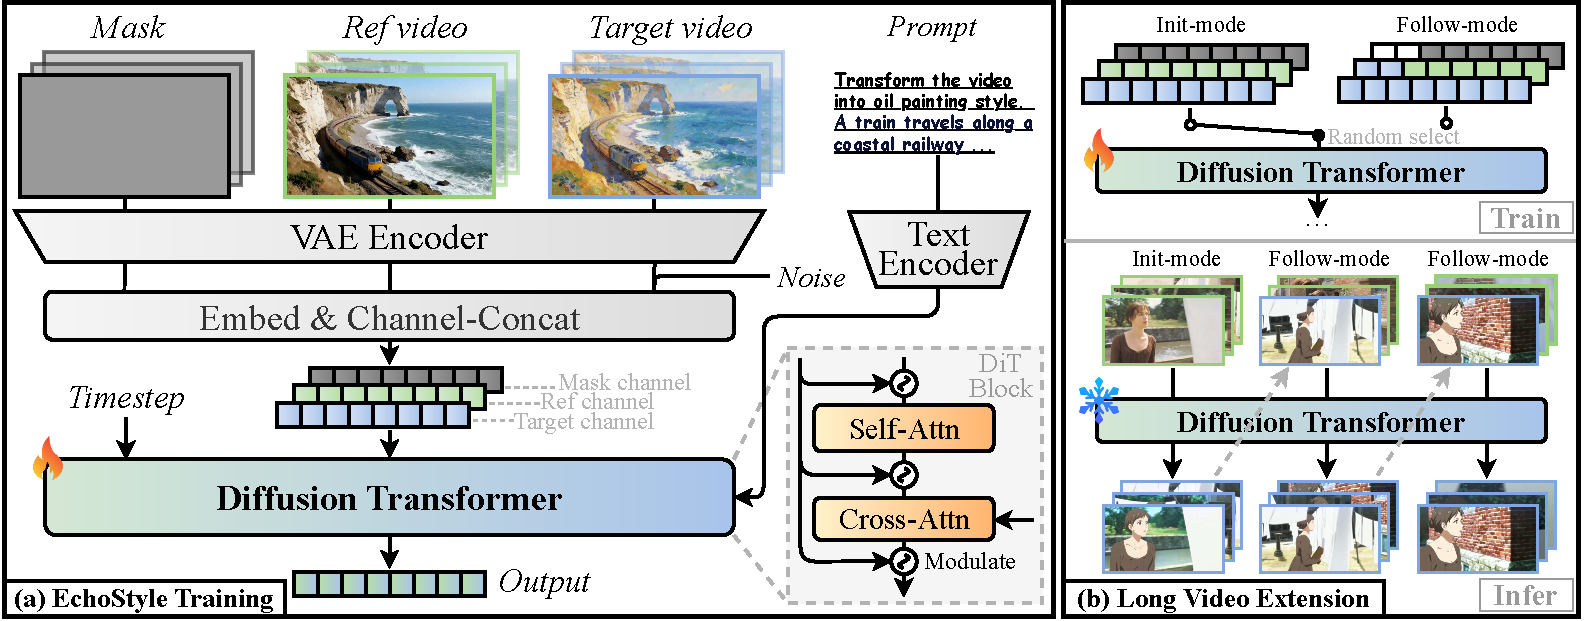
\includegraphics[width=\textwidth]{pdf/pipeline.pdf} % LaTeX自带的测试图名
    \caption{Overview of the EchoStyle framework. (a) Training: We map the mask, reference video, and target video into the shared latent space, followed by visual alignment. These multi-channel embeddings are then fed into a DiT for stylized video generation, guided by textual prompts. (b) Long Video Extension: We propose an init-follow-mode training strategy. During training, these modes are randomly selected. In the inference stage, long videos are generated autoregressively, where init-mode generates the starting sequence and subsequent segments are produced via follow-mode.}
    \label{fig:pipe}
\end{figure}
Formally, we characterize text-driven video-to-video stylization through a set of input conditions: a text prompt $p$, which encompasses both target style and content descriptions, a reference video $\mathbf{R}$ to be stylized, and a mask $\mathbf{M}$ to define which frames to be modified. We expect the model to produce the output video $\mathbf{O}$ through the mapping:
\begin{equation}
    \mathbf{O} = \Phi(\mathbf{R},\mathbf{M}, p),
\end{equation}
where $\Phi(\cdot)$ denotes the generative framework, and $\mathbf{M}$ is set to 0 for every frame.

The task of video stylization primarily hinges on addressing two core challenges: achieving rigorous content alignment with the reference video and developing expandable potential. To overcome these bottlenecks, EchoStyle adopts a streamlined yet effective architecture as illustrated in Fig.~\ref{fig:pipe}(a). To specify, we use the Variational Autoencoder (VAE)~\cite{VAE} to encode the reference video $\mathbf{R}$, the target video $\mathbf{V}$ into the latent space, yielding their respective latent representations, $\mathbf{z}_R$ and $\mathbf{z}_V$.
Next, a timestep $t$ is uniformly sampled from {1, ..., $T$}. We then corrupt the target latent $\mathbf{z}_V$ with noise according to the diffusion process forward kernel, resulting in the noisy latent $\mathbf{z}_V^{(t)}$.
% $$
% q(\mathbf{z}^{(t)}|\mathbf{z}^{(0)}) = \mathcal{N}(\mathbf{z}^{(t)}; \sqrt{\bar{\alpha}_t}\mathbf{z}^{(0)}, (1-\bar{\alpha}_t)i)
% $$
% Thus, the noisy latent $\mathbf{z}_t^{(t)}$ is obtained by:
% $$
% \mathbf{z}_t^{(t)} = \sqrt{\bar{\alpha}_t}\mathbf{z}_t + \sqrt{1-\bar{\alpha}_t}\boldsymbol{\epsilon}
% $$
% where $\boldsymbol{\epsilon} \sim \mathcal{N}(0, i)$ is a standard Gaussian noise, and $\bar{\alpha}_t$ is the cumulative product of the noise schedule.
Concurrently, $\mathbf{M}$, which shares the same spatial and temporal dimensions as the input videos, is then reshaped to match the shape of the latent $\mathbf{z}_V^{(t)}$ and $\mathbf{z}_R$, yielding $\mathbf{z}_M$. Finally, we concatenate these three latent tensors along the channel dimension to form the unified model input $\mathbf{z}_{in}$ as:
\begin{equation}
    \mathbf{z}_{\text{in}} = \text{Concat}(\mathbf{z}_R, \mathbf{z}_V^{(t)}, \mathbf{z}_M).
    \label{equ:concat}
\end{equation}
By introducing this unified and standardized visual alignment strategy, we consolidate diverse references ($\mathbf{R},\mathbf{V},\mathbf{M}$) into a unified latent. This approach ensures high semantic coherence, spatial and temporal alignments between the input video condition and the target $\mathbf{V}$.

This concatenated tensor is then fed into the backbone for noise prediction,
% 模型的主干网络由DiT模块堆叠而成。t通过adaptLN的方式注入，prompt通过T5模型token化之后，通过DiT模块内的cross-attention进行注入。所以对于短视频生成的训练来说，noise_pred = DiT(concat[za,zb',t,prompt])
%所以模型的优化目标为：最常见的noise L2损失，即为diffusion的损失公式。
which is constructed by stacking a series of Diffusion Transformer (DiT) blocks~\cite{dit}. 
The conditioning information, including the timestep $t$ and textual prompt $p$, is injected into the network through Adaptive Layer Normalization (adaLN) and Cross-Attention. The forward propagation of the DiT model can be denoted as:
\begin{equation}
    \frac{d\mathbf{z}_V^{(t)}}{dt}=\boldsymbol{\epsilon}_{\mathbf{\theta}} = \text{DiT}(\mathbf{z}_{\text{in}}, t, p),
    \label{eq:forward_pass}
\end{equation}
where $\boldsymbol{\epsilon}_{\mathbf{\theta}}$ is the prediction from our model $\mathbf{\theta}$.
% Specifically, the diffusion timestep $t$ is integrated into each DiT block via Adaptive Layer Normalization (adaLN), a technique proven effective for modulating network activations based on conditional inputs. The formulation for adaLN can be expressed as:
% \begin{equation}
%     \text{adaLN}(\mathbf{h}, t) = (\gamma_t, \beta_t) \cdot \text{LayerNorm}(\mathbf{h}),
%     \label{eq:adaln}
% \end{equation}
% where $\mathbf{h}$ is the hidden representation within a DiT block. The scale $\gamma_t$ and shift $\beta_t$ parameters are derived from $t$ through a small multi-layer perceptron (MLP).
We utilize the standard flow-matching loss as the training objective, which is to minimize the MSE between the prediction $\boldsymbol{\epsilon}_{\mathbf{\theta}}$ and the ground-truth $(\mathbf{z}_V^{(0)} - \boldsymbol{\epsilon})$, then update the entire model in a LoRA~\cite{lora} manner. The training objective can be denoted as:
\begin{equation}
    \mathcal{L}(\mathbf{\theta}) = \mathbb{E}_{t \sim \mathcal{U}[0, 1]} \left\| \frac{d\mathbf{z}_V^{(t)}}{dt} - (\mathbf{z}_V^{(0)} - \boldsymbol{\epsilon}) \right\|^2_2.
\end{equation}

% \begin{equation}
%     \mathcal{L}_{\text{diff}} = \mathbb{E}_{\mathbf{z}_b, \boldsymbol{\epsilon}\sim\mathcal{N}(0,i), t} \left[ \left\| \boldsymbol{\epsilon} - \boldsymbol{\epsilon}_{\mathbf{\theta}}(\text{Concat}(\mathbf{z}_a, \sqrt{\bar{\alpha}_t}\mathbf{z}_b + \sqrt{1-\bar{\alpha}_t}\boldsymbol{\epsilon}, \mathbf{z}_m), t, \mathbf{c}) \right\|^2_2 \right].
%     \label{eq:loss_function}
% \end{equation}

%同时，由于Wan2.2使用了moe架构来拆分采样时间步，我们分别训练了两个适配模型来保持原生的Moe架构，分别处理high-noise与low-noise时间步，从而保证对于高低频的区分处理策略，进一步提高模型性能。
%The W.A.N. 2.2 backbone employs a Mixture-of-Experts (MoE) architecture that partitions the diffusion timesteps into ``high-noise'' and ``low-noise'' regimes, each handled by specialized experts. To preserve this native design, we train two distinct sets of adapter weights. Each adapter is specialized for one regime, ensuring that the model's differentiated processing strategy for high-frequency (low-noise) and low-frequency (high-noise) information is maintained. This dual-adapter approach is crucial for leveraging the base model's full potential and further enhances generative performance.
\begin{figure}[t] % r 代表右侧, 0.4\textwidth 是图片占据的宽度
    \centering
    \includegraphics[width=\textwidth]{pdf/data_compare.pdf} % 这里的宽度通常略小于上面的宽度
    \caption{Forward vs. Reverse Data Pipelines. (a) The forward pipeline suffers from significant distribution mismatch and style drift. (b) In contrast, our reverse pipeline leverages real stylized data as the source, achieving superior distribution alignment and more robust generation results.}
    \label{fig:data_compare}
\end{figure}
\subsection{Curating High-Quality Video Pairs}
\label{sec:data_pipeline}
%数据构建放在最后面；%数据集描述
%鉴于大规模成对风格转换数据集的缺失，利用现有模型进行数据合成已成为一种普遍策略。在本文中，我们选择从收集的风格化视频反向合成真实视频作为模型的参考输入，而非正向合成风格化视频。此决策主要基于以下两点考量。

%motivation简化描述
%1.目标分布的纯粹性决定了模型的性能上限。 现有AI工具合成的风格化视频存在固有缺陷，如风格多样性有限、易产生帧间闪烁与风格漂移等问题。若将此类合成数据作为训练目标，无疑会引入噪声和偏见，严重污染目标分布，从而限制了模型的最终生成质量。诚然，我们反向合成的真实视频输入端也并非完美，但现代扩散模型（Diffusion Model）对输入端的噪声表现出强大的鲁棒性。模型的核心任务是学习从输入到目标的映射函数，只要此映射是可学习的，输入端的瑕疵在很大程度上可以被模型所适应或“过滤”。
%2.逆向利用现有模型的偏见（Bias）以提升合成质量。 在主流视频生成模型中，“风格漂移”是一个普遍存在的缺陷，即生成的风格会随时间推移和场景变化而趋向于真实风格，这源于其预训练数据集中真实风格数据占据主导地位的数据偏见。然而，在我们的反向合成任务（风格 → 真实）中，这种“缺陷”反而成为一种有利的归纳偏置。它驱使模型更稳定、更精确地生成真实风格的视频。实验证实，即使向VACE等模型输入风格化的首帧，其后续生成的帧也能有效地回归至真实风格，这为我们构建高质量的输入数据提供了有力支持。
Given the scarcity of large-scale, paired video stylization datasets, synthesizing data with existing models is a common strategy.
However, AI-synthesized stylized videos suffer from limited stylistic diversity, flickering, and style drift. As Fig.~\ref{fig:data_compare} illustrates, using such data as a training target would contaminate the objective distribution with these flaws, thereby capping the model's potential. This limitation stems from the data bias inherent in current video2video tools, where the training sets are dominated by real-world imagery. 

We effectively address the aforementioned challenges by inverting the direction of this synthesis process. To specify, we collect authentic stylized videos and synthesize their corresponding realistic counterparts to serve as source inputs. 
The primary advantage of this approach lies in defining authentic stylized videos as the target distribution, which ensures the purity of the learning objective and effectively circumvents the performance bottlenecks typically imposed by synthetic artifacts or stylistic drift. 
Furthermore, by strategically exploiting the intrinsic realism bias of pre-trained models, we achieve superior fidelity and stability in reference video construction during reverse synthesis, utilizing model bias as an advantage for high-quality data curation.

\begin{figure}[t]
    \centering
    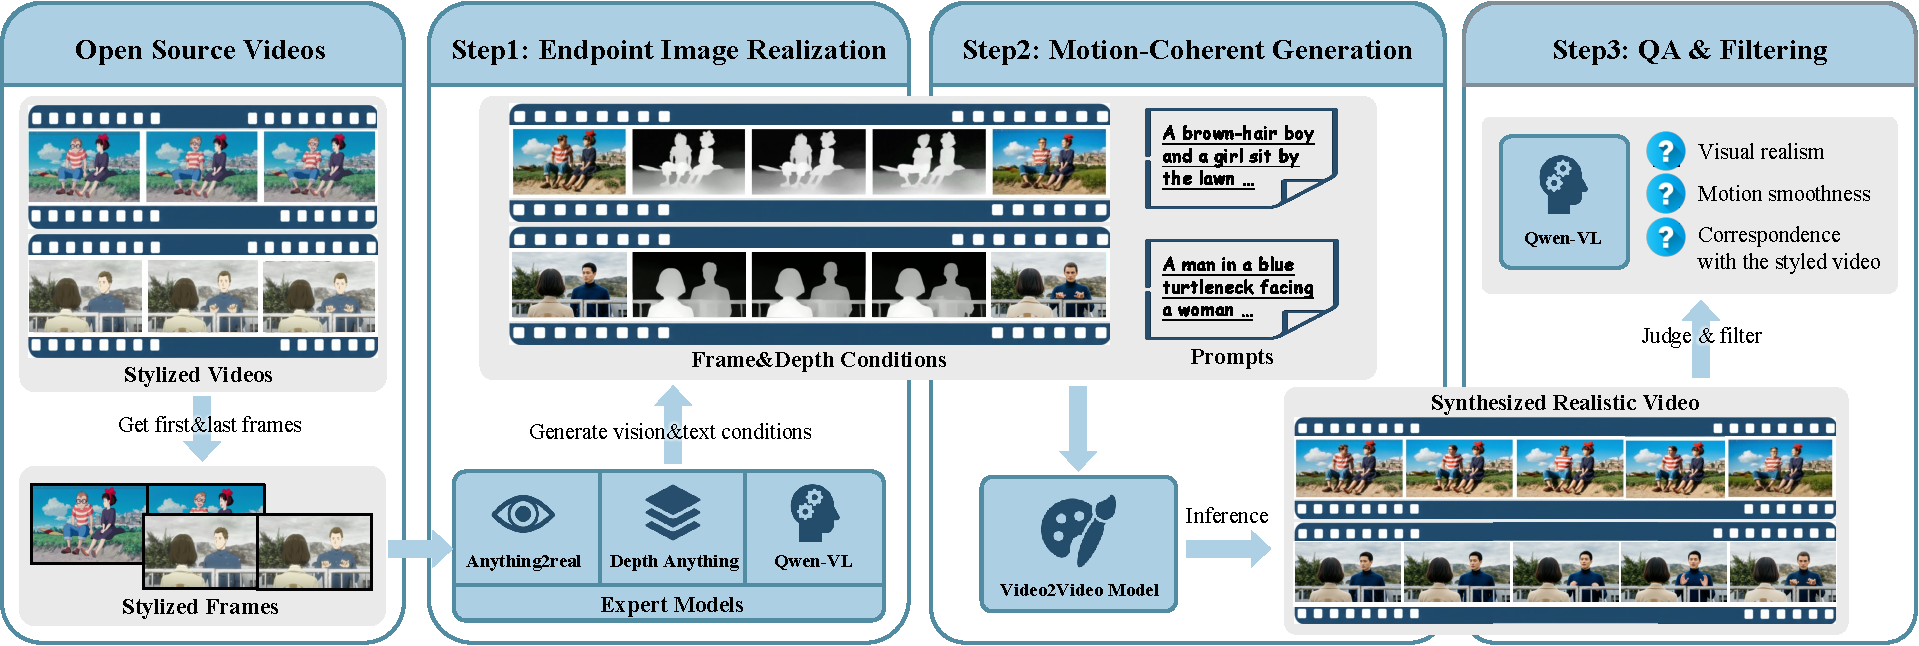
\includegraphics[width=\textwidth]{pdf/data_pipe.pdf} % LaTeX自带的测试图名
    \caption{Our data synthesis pipeline is organized into three stages: first, endpoint image stylization establishes the style for boundary frames; second, motion-coherent V2V generation produces semantically-aligned video sequences; and finally, automated filtering via VLMs is employed to vet video quality and discard suboptimal samples.}
    \label{fig:data_pipe}
\end{figure}
%Given the scarcity of large-scale, paired video stylization datasets, synthesizing data with existing models is a common strategy. However, instead of synthesizing stylized videos from real ones (real-to-stylized), we propose a \textit{reverse synthesis} approach: we collect authentic stylized videos and synthesize their corresponding realistic counterparts to serve as source inputs. This design choice is motivated by two key considerations.

%\noindent\textbf{Maintaining the purity of the target distribution.}
%The performance ceiling of a generative model is dictated by the quality of its target distribution. AI-synthesized stylized videos suffer from inherent artifacts, such as limited stylistic diversity, flickering, and style drift. Using such data as a training target would contaminate the objective distribution with these flaws, thereby capping the model's potential. Conversely, while our synthesized \textit{source} videos may also have imperfections, diffusion models are robust to noise in the input domain. The model's task is to learn a mapping to a pristine, high-quality target distribution (authentic stylized videos), a process where input-level noise can be effectively filtered or adapted to.

%\noindent\textbf{Leveraging Model Bias for Data Fidelity.}
%A common failure mode in existing video generation models is ``style drift''---a tendency to revert to realism over time. This is a direct consequence of the data bias in their pre-training, which is dominated by real-world footage. We strategically exploit this bias. In our reverse synthesis task (stylized $\rightarrow$ real), this "flaw" becomes a beneficial inductive bias, compelling the generator to produce more stable and realistic source videos. Empirical evidence confirms this; for instance, even when conditioned on a stylized initial frame, models like VACE~\cite{vace_reference} quickly converge to generating realistic subsequent frames, providing a robust mechanism for creating high-quality source data for our pipeline.

% 突出重点；V2V架构；拼接方式；公式

%我们的数据处理框架主要遵循以下流程：从open-source中获取style video（多为影视或动漫剪辑），然后将其裁取首尾帧集合。我们使用qwen-image与anything2real-lora作为真实图像生成的expert，将裁取的style图像转化为真实照片图像。然后，我们使用VACE作为视频转视频的expert生成真实视频，为了遵循与style video相同的运动模式，我们从style video提取深度视频，并在其首尾帧插入转绘之后的真实图像，作为视频转视频expert的condition进行生成。在获取pair视频对之后，我们引入qwen-VL模型进行评测与检查，判断生成视频的真实度，运动幅度，以及与目标视频的细粒度对应。
As shown in Fig.~\ref{fig:data_pipe}, our automated data collection pipeline proceeds as follows:
\begin{itemize}
\item \noindent\textbf{Stylized Video Collection.} We collect stylized video clips from open-source datasets and extract their initial and final frames.
    \item \noindent\textbf{Image Realization.}
We translate the first and final frames of the stylized videos into realistic endpoint anchors using Qwen-Image~\cite{qwenimage} as the base model and Anything-to-Real LoRA for image-to-image translation. 
\item \noindent\textbf{Motion-coherent V2V Generation.} These transformed realistic images, combined with depth priors extracted from the original stylized clip, serve as conditions for VACE~\cite{jiang2025vace}. This depth and first \& last frame-guided process ensures the generated realistic video maintains precise content coherence with the stylized video.
\item \noindent\textbf{Quality Assessment.}
To ensure data fidelity, we utilize Qwen-VL~\cite{qwenvl} to screen video pairs based on three key metrics: (i) generated visual realism, (ii) motion plausibility, and (iii) fine-grained temporal correspondence. Only pairs that meet these rigorous criteria are incorporated into the final training dataset.
\end{itemize}

\textit{V-Style20k} \textbf{Dataset.} 
%在反向数据pipeline的基础上，我们构建了一个风格配对视频数据集，用以支持视频风格化的相关研究。该数据集由480p分辨率的视频组成，长度为5s以内。数据集共收集了14种用于影视动漫或艺术领域的常见风格，并采用qwen-vl进行了文本标注。
Leveraging this reverse data pipeline, we establish \textit{V-Style20k}, a large-scale paired video dataset designed to facilitate research in video stylization. The dataset comprises over 20,000 high-quality video pairs at a resolution of 480×832, with each clip restricted to a duration of under 5 seconds. \textit{V-Style20k} encompasses 14 diverse styles prevalent in cinematography, animation, and fine arts. Furthermore, to support text-driven tasks, each sample is meticulously annotated with descriptive captions using the Qwen-VL~\cite{qwenvl} vision-language model.
We formally denote our dataset $D$ as:
\begin{equation}
    D = \{(p_j, \mathbf{R}_j, \mathbf{V}_j, \mathbf{T}_j)|j=1,2,\dots,N\}.
\end{equation}
Specifically, each data sample comprises a text prompt $p$ describing the intended style and content, an input reference video $\mathbf{R}$ serving as the content prior, a target stylized video $\mathbf{V}$, and a $\mathbf{T}$ serving temporal condition which will be thoroughly discussed in Sec.~\ref{sec:long_video}. We provide the illustration and statistics of our dataset in Fig.~\ref{fig:dataset}.
\begin{figure}[t]
    \centering
    \includegraphics[width=\textwidth]{pdf/dataset.pdf}
    \caption{Representative samples and statistical characterization of V-Style20k.}
    \label{fig:dataset}
\end{figure}

\subsection{Expanding to Long-Video Stylization}
\label{sec:long_video}

%为解决长视频生成中普遍存在的显存瓶颈问题，并实现可拓展的视频风格迁移，我们设计了一种基于滑动窗口的自回归（autoregressive）生成框架。

%改为motivation
%传统的自回归扩散模型通常以前一帧的生成结果为条件来预测下一帧。EchoStyle借鉴并扩展了此思想，将自回归的单元从“帧”（frame）提升至“视频片段”（clip）。在推理阶段，待处理的长视频被分割成一系列重叠的视频片段。模型以序列化的方式处理这些片段，将前一个已处理片段的输出作为时序引导条件，来生成下一个片段。这种策略将计算复杂度和显存占用控制在恒定且可管理的范围内，从而理论上支持对无限长度视频（infinite-length video）的风格迁移。我们的实验证实，该方法可稳定地将视频转绘任务拓展至分钟级别。

%给推理细节
%具体实现细节如下：我们构建了一个统一的框架来处理短视频与长视频的生成任务。如章节3.2所述，我们引入了一个单通道的二进制掩码（binary mask），其维度与视频张量相同，用于指示模型是否需要对特定帧进行修改。为了赋予模型时序拓展的能力，我们在训练阶段进行了特定的数据增强。具体而言，我们将目标视频（target video）的初始片段（例如前 k 帧）截取出来，并用它替换参考视频（reference video）对应位置的内容。这样便构造了一个包含历史风格化信息的**“时序-结构混合引导视频”**（Temporal-Structural Hybrid Condition）。同时，我们将原本全为0的掩码张量中，对应于该引导片段的部分置为1。这个掩码向模型明确指示：这部分内容是已知的上下文，无需进行重绘。在推理阶段，这种自回归机制被激活。第一个视频片段的时序引导信息为空（或使用特定初始帧），生成输出后，该输出的末尾片段便成为下一个视频片段的时序引导信息，如此循环往复，从而实现了平滑且一致的长视频生成。

% 为解决长视频生成中普遍存在的显存瓶颈问题，并实现可拓展的视频风格化，我们设计了一种基于滑动窗口的，基于temporally recurrent multi-frame token mechanism的生成框架。我们通过将占用较多推理资源的长视频转变为若干可以迭代处理的视频clip，从而将显存占用上限规范到可控范围；同时，通过引入多帧时序条件可以有效将长短视频融合到统一框架中，提高了简洁性和运行成本。
%具体而言，在训练时，我们将目标视频（target video）的初始片前 k 帧截取出来，并用它替换参考视频（reference video）对应位置的内容。这样便构造了一个包含历史风格化信息的“时序-结构混合引导视频”（Temporal-Structural Hybrid Condition）。同时，我们将原本全为0的掩码张量中，对应于该引导片段的部分置为1。这个掩码向模型明确指示：这部分内容是已知的上下文，无需进行重绘。在推理阶段，这种自回归机制被激活。第一个视频片段的时序引导信息为空，生成输出后，该输出的末尾片段（后k帧）便成为下一个视频片段的时序引导信息，如此循环往复，从而实现了平滑且一致的长视频生成。这个过程可以被表示为：
To mitigate the pervasive memory bottlenecks in long-video generation and achieve expandable stylization, we propose a sliding-window-based generation framework powered by an init-follow-mode mechanism during training, as shown in Fig.~\ref{fig:pipe}(b). Specifically in the follow mode, we introduce a temporal reference video $\mathbf{T}$, which is constructed by replacing the initial $x$-frame window of $\mathbf{R}$ with the corresponding stylized frames from $\mathbf{V}$. During training, we utilize VAE to compress $\mathbf{T}$ into $\mathbf{z}_T$. Then we replace $\mathbf{z}_R$ in Eq.~(\ref{equ:concat}) with $\mathbf{z}_T$ to realize dual-mode training, and modify the respective frames in the mask $\mathbf{M}$ as 1 to indicate that these frame need to be preserved, which can be denoted as:
\begin{equation}
    \mathbf{z}_{\text{in}} = \text{Concat}(\mathbf{z}_T, \mathbf{z}_V^{(t)}, \mathbf{z}_M).
\end{equation}
In each training iteration, we choose $\mathbf{z}_{\text{in}}$ from two modes with a fixed probability, ensuring the network effectively balancing its capacity.

During inference, instead of relying solely on the first frame, we utilize clip-guided conditioning to reduce the sensitivity to one single frame's quality and enhance the temporal stability of the stylized output. We partition the long-form video into a sequence of shorter segments $\{\mathbf{R}_{0}, \mathbf{R}_{1}, \dots, \mathbf{R}_{n}\}$, where each consecutive pair $(\mathbf{R}_{i}, \mathbf{R}_{i+1})$ shares a temporal overlap of $x$ frames.
% , effectively bounding the peak GPU memory to a controllable range, regardless of the total video length.
The initial segment $\mathbf{R}_{\mathbf{0}}$ is processed following the short-duration pipeline. 
For subsequent segments $\mathbf{R}_{i}$ ($i > 0$), the generation is conditioned on the overlapping stylized frames from the previous output $\mathbf{O}_{i-1}$. 
Formally, let $\mathbf{O}_{i-1}[-x:]$ denote the last $x$ frames of the preceding stylized segment. $\mathbf{M}_x$ means setting the first $x$ frames of $\textbf{M}$ to 1 to indicate that these frames should be modified. The inference for $\mathbf{R}_{i}$ is formulated as:
\begin{equation}
    \mathbf{O}_{i} = \Phi(\mathbf{R}_{i},\mathbf{M}_x, p_{i}, \mathbf{O}_{i-1}[-x:]),
\end{equation}
This process ensures smooth and temporally coherent generation across long video sequences. The equation can be formulated as:
\begin{equation}
\mathbf{O}_{\text{long}} = \mathbf{O}_0 \mathbin{\Vert} \sum_{i=1}^{n} \mathbf{O}_i[x:].
\end{equation}
where $\mathbin{\Vert}$ denotes the concatenation operator along the temporal axis. This init-follow-mode mechanism helps us to seamlessly integrate both training and inference process in variable-length video stylization into a unified pattern, not only enhancing the structural simplicity but also significantly reducing computational costs associated.
    

%To address the significant memory constraints inherent in long-video processing and to enable scalable stylization, we introduce a sliding-window, autoregressive framework.

%\noindent\textbf{Autoregressive Clip-based Generation.}
%Inspired by traditional autoregressive diffusion models that condition on previous frames, our approach elevates this concept from a frame-level to a clip-level. During inference, a long video is divided into a sequence of overlapping clips. The model processes these clips sequentially, where the output of a preceding clip serves as the temporal condition for generating the subsequent one. This strategy maintains a constant and manageable memory footprint, theoretically enabling stylization of videos of infinite length. Our experiments validate that this method can stably extend video stylization to minute-long durations.

%\noindent\textbf{Training and Implementation.}
%We employ a unified framework for both short- and long-video tasks. As detailed in Sec.~\ref{sec:v2v_network}, a binary mask $\mathbf{M}$ is used to designate which frames require modification. To equip the model with temporal extension capabilities, we introduce a specific training data augmentation. We construct a \textit{temporal-structural hybrid condition} by replacing the initial segment of the source video with the corresponding stylized segment from the target video. Concurrently, the mask values for this segment are set to 1, instructing the model to treat these frames as known context and not redraw them.

%During inference, this autoregressive mechanism is activated. The stylized tail of a generated clip becomes the conditioning head for the next, forming a recurrent loop. This process ensures smooth and temporally coherent generation across long video sequences.



%\noindent\textbf{1. Endpoint Image Realization.}
%We employ a set of expert models for image-to-image translation. Specifically, we use Qwen-VL~\cite{qwen_vl_ref} for semantic understanding and an Anything-to-Real LoRA~\cite{anything2real_ref} to translate the stylized frames into realistic photo-style images.

%\noindent\textbf{2. Motion-Coherent Video Synthesis.}
%Next, we use VACE~\cite{vace_ref} as our video-to-video synthesis expert to generate the full realistic source video. To ensure the synthesized video follows the precise motion patterns of the original stylized clip, we provide VACE with a specialized condition. This condition is constructed by first extracting a depth video sequence from the original stylized video. We then insert the newly synthesized realistic images (from Step 1) as the start and end frames of this depth sequence. This depth-and-endpoint-conditioned input guides VACE to generate a motion-coherent, realistic video.

%\noindent\textbf{3. Quality Assurance and Filtering.}
%Upon generating a candidate video pair, we perform an automated quality assurance step. We leverage the Qwen-VL~\cite{qwen_vl_ref} model as an evaluator to assess the generated source video based on three criteria: (1) degree of realism, (2) motion magnitude and plausibility, and (3) fine-grained temporal correspondence with the target stylized video. Pairs that pass this rigorous inspection are added to our final training dataset.

% data pipeline
% framework
% auto-regressive generation
\section{Experiment}
\subsection{Implementation Details}
% 数据准备。我们使用独有的数据curation pipeline构造了V-Style20k数据集，共包含18k视频对，原始尺寸为480*832。在训练时，统一裁剪到480*480进行处理。时间长度/帧数采用 bucket 策略，最小帧数为33，最大为69，以16FPS进行训练。
% 基础模型与组件. 我们在 Wan2.2 I2V 14B 的high noise与low noise预训练权重上进行微调，训练中 冻结 VAE 与文本编码器，仅更新 DiT 上插入的 LoRA 参数，在所有 nn.Linear 层上注入 rank 为 64，lora_alpha=32的lora，并以 Gaussian 初始化。训练通过 torchrun 启动，随机种子设置为 seed=42，单卡batch_size为1，并按 seed+rank 做多进程去相关；每一个模型均在16卡A100上做20000步训练，耗费120h。
% 训练策略。在训练时，每次迭代提供多种文本/视频条件的组合采样。以 0.8 概率使用完整文本条件（转绘指令与画面内容描述的集合），否则使用粗略文本（仅指令）。同时，以 0.8 概率使用原始参考视频并置零 mask；以 0.2 概率添加自回归视频拓展条件，并对序列开头位置施加显式 mask，用于强化起始片段约束，训练长视频推理。同时我们使用混合精度训练，为减少推理分支开销，非 LoRA 权重被转换为 bfloat16。使用使用AdamW优化器进行梯度优化betas=(0.9,0.999), weight_decay=0.01, eps=1e-8，设置学习率为恒定常数2e-5。

\textbf{Data Preparation.} 
To facilitate our training process, we utilize \textit{V-Style20k} during our training process. Videos are center-cropped to a spatial resolution of $480 \times 480$ to maintain consistency. We adopt a temporal bucket strategy to handle varying sequence lengths, with frame counts ranging from 33 to 69 frames, all sampled at a frame rate of 16 FPS.

\textbf{Base Model and Components.} 
Our framework is initialized with the pre-trained weights of Wan2.2-I2V-14B, spanning both high-noise and low-noise regimes. During the fine-tuning stage, we freeze the VAE and text encoders, updating only the LoRA parameters integrated into the DiT backbone. Specifically, we inject LoRA into all \texttt{nn.Linear} layers with a rank of $r=64$ and $\alpha=32$, utilizing Gaussian initialization. Training is orchestrated via torchrun on a cluster of 16 NVIDIA A100 GPUs. We set the global seed to 42 and apply a per-GPU batch size of 1, utilizing a $seed+rank$ strategy to ensure multi-process decorrelation. The model is trained for $20,000$ steps, totaling approximately 80 hours of computation.
% Please add the following required packages to your document preamble:
% \usepackage[normalem]{ulem}
% \useunder{\uline}{\ul}{}

\textbf{Training Strategy.} 
To enhance the model's robustness and controllability, we employ a diverse sampling strategy for text and video conditioning during each iteration. For textual guidance, the model is provided with full captions (a concatenation of style instructions and content descriptions) with a probability of 0.8; otherwise, only style instructions are used. 
Regarding visual conditioning, we utilize reference video $\mathbf{R}$ with all-zero mask $\mathbf{M}$ in 80\% of the samples. For the remaining 20\%, we use temporal reference video $\mathbf{T}$ with the modified mask $\mathbf{M}_x$, and $x$ is set to 16 during training. 
We leverage mixed-precision training, where non-LoRA weights are converted to \texttt{bfloat16} to reduce memory overhead. Optimization is performed using the AdamW optimizer with $\beta=(0.9, 0.999)$, a weight decay of $0.01$, and a constant learning rate of $2 \times 10^{-5}$.
%为了与其他开源与闭源方法进行对比，我们收集网络视频，构造了一个50对指令-输入，图文对应的测试集，测试集中共包含9种常见风格，我们将其与视频进行随机配对。由于基于文本指令的视频风格编辑到目前为止并无开源方法，我们选取了Runway，Kling-O1与Seedance2.0这三个商业闭源模型进行对比，并选取VACE，anyV2V作为开源模型的对比方法，由于这两个模型并不支持文本编辑功能，仅支持首帧引导生成，我们将测试集视频的第一帧输入qwen-image进行风格化，再输入模型pipeline种进行处理。
\subsection{Comparison Experiment}
To benchmark our method against both open-source and closed-source models, we assemble an evaluation set of 50 video-instruction pairs featuring nine representative styles. Due to the scarcity of text-based video editing open-source tools, we compare our model with leading commercial solutions (Runway, Kling-O1~\cite{Kling-O1}, and Seedance 2.0~\cite{seedance2.0}) and open-source V2V baselines (VACE~\cite{jiang2025vace} and AnyV2V~\cite{kuanyv2v}). To bridge the functional gap of the open-source V2V models, which support frame-conditioned generation, we utilize Qwen-Image~\cite{qwenimage} to stylize the first frame as a reference guide, ensuring a consistent and fair evaluation across different modalities.

%在定量指标方面，我们共衡量三个标准：风格转绘质量，视频质量，与人类偏好评估。在风格转绘质量方面，我们选取csd score，计算视频与参考风格图（图像来自于相关风格影片的网络收集）的风格相似度；同时，我们通过衡量每一帧与首帧的风格相似度来量化风格一致性。在视频质量方面，我们follow VBench中的相关设置，评估'background_consistency', 'motion_smoothness', 'dynamic_degree', 'aesthetic_quality', 'imaging_quality'这五个指标。在人类偏好评估中，我们评分视频的美学质量，以及与输入视频的细粒度对齐（内容一致性）。

Quantitative evaluations are performed across three dimensions: style quality, video quality, and human preference. 
% 我们使用VLM评测的方式来衡量Style Similarity，我们使用两两组对的方式使模型判断哪个方法更接近给定风格，并统计每个方法的胜率。同时，我们使用csd得分来计算每一帧与第一帧之间的风格相似度，从而衡量style consistency.
To evaluate style similarity, we leverage Gemini-3-pro~\cite{team2023gemini} to perform automated pairwise comparisons. Specifically, for each test case, the model is tasked with identifying which generated video aligns more closely with the reference style; the performance of each method is then quantified by its overall win rate. 
Furthermore, we assess style consistency by calculating the CSD scores~\cite{csd} between each subsequent frame and the initial frame. This metric serves to measure the stylistic stability across the temporal dimension, ensuring that the stylistic attributes remain coherent throughout the video sequence.
Following the established settings of VBench~\cite{huang2024vbench}, we assess video quality through motion smoothness and imaging quality. In addition to standard metrics, we employ Gemini-3-pro~\cite{team2023gemini} to perform a comprehensive automated assessment of the results, focusing on dynamic quality, static quality, and quality. Furthermore, our human preference evaluation focuses on both artistic scores and fine-grained content alignment with the input videos. We refer the reader to the Supplementary Material for more details.

\begin{table}[t]
\centering
\caption{Quantitative comparison between EchoStyle and SOTA methods. The \textbf{best} and \underline{second-best} results are highlighted in \textbf{bold} and \underline{underline}, respectively.}
\label{tab:comparison}

% 1. 增加行高，防止文字挤在横线上
\renewcommand{\arraystretch}{1.3} 
% 2. 稍微增加线条粗细（可选，默认0.4pt，这里设为0.6pt）
\setlength{\arrayrulewidth}{0.4pt}
% 3. 调整列间距
\setlength{\tabcolsep}{4pt}
\begin{adjustbox}{max width=0.95\textwidth}
\begin{tabular}{c|cc|ccccc}
\noalign{\hrule height 1pt}
& \multicolumn{2}{c|}{Style Quality} & \multicolumn{5}{c}{Video Quality} \\ \hline
Method & \makecell{Style\\Similarity} & \makecell{Style\\Consis.} & \makecell{Motion\\Smooth.} & \makecell{Imaging\\Qual.} & \makecell{Static\\Qual.} & \makecell{Dynamic\\Qual.} & \makecell{Aesthetic\\Qual.} \\ \noalign{\hrule height 1pt}
AnyV2V      & 0.351 & \underline{0.877} & 0.957 & 0.654 & 0.733 & 0.611 & 0.815 \\
VACE-Depth  &0.280 & 0.805 & 0.972 & 0.687 & 0.845 & 0.700 & 0.837 \\
VACE-Flow   &0.394 & 0.819 & 0.960 & 0.681 & 0.856 & 0.732 & 0.852 \\ \hline
Runway      & 0.239 & 0.860 & \underline{0.982} & 0.704 & 0.721 & 0.637 & 0.747 \\
Kling-O1    & \textbf{0.809} & 0.883 & \textbf{0.984} & \textbf{0.746} & \textbf{0.879} & \underline{0.775} & 0.806 \\
Seedance2.0 & 0.628 & 0.831 & 0.980 & \underline{0.725} & \underline{0.860} & 0.741 & \textbf{0.885} \\ \hline
EchoStyle   & \underline{0.802} & \textbf{0.895} & 0.966 & 0.696 & 0.850 & \textbf{0.783} & \underline{0.878} \\ \noalign{\hrule height 1pt}
\end{tabular}
\end{adjustbox}
%\vspace{-5mm}
\end{table}

%对比实验的定性与定量结果如图a，b与表c所示，从定量指标来看，echostyle与对比方法相比，整体上表现最优，在风格转绘效果与人类感知评估中均取得了sota，在视频质量方面，我们取得了最优的aesthetic_quality与dynamic_degree，但在其他三个指标中差于商业闭源模型。从定性结果对比来看，kling-o1与Seedance2.0，尽管有较高的视觉质量，但无法做到帧级对应的细粒度对齐，同时kling-o1生成复杂场景的能力较弱，画面细节较少。Runway能够做到细粒度的对齐，但整体画面质量与表现力较差，并不能成功修改至期望风格。VACE与AnyV2V这种基于首帧引导的方法，在处理突然出现或者激烈运动时表现较差，VACE出现了风格丢失问题，而anyV2V的预设中无法处理16帧以上的视频人物。综合相比，echostyle在风格转绘质量，视频质量，与人类偏好评估均取得最优。

The qualitative and quantitative comparisons are summarized in Fig. \ref{fig:compare}, Tab.~\ref{tab:comparison} and Tab.~\ref{tab:hp}. In summary, EchoStyle demonstrates superiority over existing baselines in style quality and human preference. Regarding video quality, EchoStyle follows closely behind SOTA closed-source methods, Kling-O1 and Seedance 2.0. Significantly, we secure the top-tier ranking in dynamic quality and the second-highest score in aesthetic quality, highlighting the immense artistic utility and excellent temporal quality of our proposed method and offering a powerful alternative for professional-grade artistic video production.

\begin{figure}[!t]
    \centering
    % 第一张图
    \includegraphics[width=\textwidth]{pdf/com.pdf} 
    \\[10pt] % 这里的 10pt 可以调节两张图之间的垂直间距
    % 第二张图
    \includegraphics[width=\textwidth]{pdf/com2.pdf}
    \caption{\textbf{Visual comparison of video stylization results.} EchoStyle demonstrates excellent visual quality and stronger temporal coherence.}
    \label{fig:compare}
\end{figure}

\begin{wraptable}{r}{7.5cm} % {r} 表示靠右，{7.5cm} 是表格占据的宽度
%\vspace{-10mm}
\centering
\caption{Comparison of Human Preference. The \textbf{best} and \underline{second-best} results are highlighted in \textbf{bold} and \underline{underline}, respectively.} % 如果需要标题，放在这里
\label{tab:hp}
\renewcommand{\arraystretch}{1.3} 
\small % 环绕表通常建议调小一点字号，防止由于太宽导致左侧文字太碎
\begin{adjustbox}{max width=0.55\textwidth}
\begin{tabular}{cccc}
\noalign{\hrule height 1pt}
method & \makecell{Style\\ Similarity} & \makecell{Style\\ Consistency} & \makecell{Content\\ Preservation} \\ \noalign{\hrule height 1pt}
AnyV2V         & 0.490                                                      & 0.768                                                            & 0.790                                                        \\
VACE-Depth     & 0.489                                                      & 0.779                                                         & 0.850                                                     \\
VACE-Flow      & 0.472                                                      & 0.765                                                   & 0.855                                                     \\\hline
Runway         & 0.386                                                      & 0.849                                                         & 0.844                                                     \\
Kling-O1        & \underline{0.815}                                                      & \underline{0.853}                                                         & 0.833                                               \\
Seedance2.0    & 0.792                                               & 0.821                                                        & \textbf{0.889}                                                     \\ \hline

EchoStyle & \textbf{0.826}                                            & \textbf{0.870}                                                & \underline{0.860}                                            \\ \noalign{\hrule height 1pt}
\end{tabular}
\end{adjustbox}
%\vspace{-5mm}
\end{wraptable}
Although Kling-O1 and Seedance 2.0 offer high visual quality, they exhibit several drawbacks in the task of fine-grained video stylization. As shown in the bottom two subfigures of Fig.~\ref{fig:compare}, Kling-O1 exhibits limited capacity in synthesizing complex scenes, often resulting in sparse details. Its generated results exhibit monotonous color schemes and simplistic lighting hierarchies, leading to lower human-rated style similarity compared to our method. Runway, while preserving alignment, suffers from suboptimal visual quality and limited expressiveness, failing to faithfully transition to the target styles. 
Seedance 2.0 achieves the best results in terms of human preference for content preservation. However, as shown in the top two subfigures of Fig. ~\ref{fig:compare}, it often struggles to maintain \textit{high-frequency stylistic details}, such as those in oil painting and ink art styles. Furthermore, we observe that its output is prone to \textit{style decoupling} between the subject and the background, as illustrated in Fig.~\ref{fig:compare} bottom-left case.
For first-frame-guided baselines, VACE experiences significant ``style loss". 
As the video progresses, the stylized features increasingly revert to their realistic counterparts.
In the stylized output, the stylistic attributes are progressively lost, converging towards the original, non-stylized frames.
Additionally, AnyV2V is constrained by its architecture to sequences under 16 frames. In summary, EchoStyle consistently outperforms competing methods across style quality, video aesthetics, and human preference evaluation.

\begin{figure}[!t]
%%\vspace{-2mm}
    \centering
    \includegraphics[width=\textwidth]{pdf/long_com1.pdf} 
    \\[10pt] % 这里的 10pt 可以调节两张图之间的垂直间距
    % 第二张图
    \includegraphics[width=\textwidth]{pdf/long_com2.pdf}
    \caption{Visual demonstration of temporally consistent stylization on extended video sequences. Our method demonstrates superior performance in maintaining content preservation, illumination depth, and artistic texture.}
    \label{fig:long_com}
    %%\vspace{-2mm}
\end{figure}

\subsection{Long Video Extension}
% 针对长时序视频生成中的内容保持与质量退化挑战，我们系统性地考察了本框架的处理能力。实验素材来源于高质量的影视长镜头，此类素材因其复杂的空间运动和光影变化，对生成的稳定性提出了极高要求。通过与当前先进模型 Kling-o1 的横向对比，我们量化了本方法在风格忠实度与长效一致性方面的优势。此外，为进一步验证生成结果的感知质量，我们还引入了人类偏好图谱。如表 a 与图 b 的实验数据所示，本方法在多个指标上均表现出卓越的竞争力。
To address the inherent challenges of content preservation and quality degradation in long-duration video generation, we systematically evaluate the robustness of our framework. 
Our experiments utilize high-quality cinematic long shots characterized by complex spatial dynamics and intricate illumination variations, which impose stringent requirements on temporal stability. 

For comparison, we employ Kling-O1 as the baseline. Specifically, for its long-duration extension, we utilize the last frame of the preceding video segment in conjunction with the reference video as conditioning prompts. The qualitative results are presented in and Fig.~\ref{fig:long_com}. Both models successfully achieve the target stylistic transformation, characterized by exaggerated facial features (e.g., enlarged eyes) and smoothed skin textures typical of modern 3D animation. However, EchoStyle demonstrates superior stylistic distillation and visual refinement, while Kling-O1 tends to produce overly simplified textures and flatter lighting. At the same time, Kling-O1 occasionally suffers from semantic drift, leading to quicker error accumulation, which causes the character motions and environmental scenes in the latter stages of the video to deviate significantly from the original source content.
% \begin{table}[t]
% \centering
% \caption{Quantitative comparison between EchoStyle and Kling-O1 in long-video stylization.}
% \label{tab:long_com}
% \begin{tabular}{c|c|ccccc}
% \noalign{\hrule height 1pt}
% \multicolumn{1}{c|}{}       & \multicolumn{1}{c|}{Style Quality\rule{0pt}{1em}}                                                                               & \multicolumn{5}{c}{Video Quality}                                                                                                                                                                                                                                                                                                                                                                                \\ \hline
% \multicolumn{1}{c|}{Method} & \multicolumn{1}{c|}{\begin{tabular}[c]{@{}c@{}}Style\\ Consistency\end{tabular}} & \multicolumn{1}{c}{\begin{tabular}[c]{@{}c@{}}Motion\\ Smoothness\end{tabular}} & \multicolumn{1}{c}{\begin{tabular}[c]{@{}c@{}}Imaging\\ Quality\end{tabular}} & \multicolumn{1}{c}{\begin{tabular}[c]{@{}c@{}}Static\\ Quality\end{tabular}} & \multicolumn{1}{c}{\begin{tabular}[c]{@{}c@{}}Dynamic\\ Quality\end{tabular}} & \multicolumn{1}{c}{\begin{tabular}[c]{@{}c@{}}Aesthetic\\ Quality\end{tabular}} \\ \noalign{\hrule height 1pt}
% Kling-O1 \rule{0pt}{1em}                                            & \textbf{0.799}                                                                   & \textbf{0.988}                                                                  & \textbf{0.767}                                                                & 80.00                                                                        & 54.00                                                                         & 82.50                                                                           \\
% EchoStyle                                  & 0.742                                                                            & 0.963                                                                           & 0.614                                                                         & \textbf{90.00}                                                               & \textbf{92.00}                                                                & \textbf{88.50}                                                                  \\ \noalign{\hrule height 1pt}
% \end{tabular}
% \end{table}
% \subsection{Zero-shot Inference}
% %\begin{wrapfigure}{r}{0.6\textwidth} % r 代表右侧, 0.4\textwidth 是图片占据的宽度
% \begin{figure}[t]

%     \centering
%     \includegraphics[width=\textwidth]{pdf/merge.pdf} % 这里的宽度通常略小于上面的宽度
%     \caption{Qualitative visualization of zero-shot generalization in multi-style blending.}
%     \label{fig:zero}
    
% \end{figure}

%\end{wrapfigure}
% 旨在进一步拓宽风格编辑的多样性并提升交互式体验，本研究深入评估了模型在复杂风格融合任务中的泛化性能。实验结果（详见图3）有力地证明了该模型具备极佳的可扩展性：通过在文本提示（Text Prompt）中引入多个风格触发词，模型能够精准解析并有效响应此类复合型文本指令。这表明模型不仅能够识别单一风格，还能在潜空间中实现多种风格属性的平滑迁移与解耦整合。
% Aiming to extend the boundaries of style editing and improve user-model interactivity, we investigate the framework’s robustness in multi-attribute blending scenarios. The results in Fig.~\ref{fig:zero} highlight the superior extensibility of our approach. By leveraging compositional prompts with multiple trigger words, the model effectively decodes and executes complex stylistic commands. This indicates that the model has learned a well-structured latent space where distinct stylistic features can be harmoniously fused and disentangled, allowing for high-fidelity synthesis of hybrid styles.
\subsection{Ablation Study}
%controlnet lora对比
\begin{figure}[t]
    \centering
    \includegraphics[width=\textwidth]{pdf/ab.pdf}
    \caption{Qualitative ablation study of model framework and temporal conditioning.}
    \label{fig:ab}
\end{figure}

%我们设计了若干消融实验来证明相应方法设计的有效性，更多实验细节请参考补充材料。

%模型框架消融。我们选用了ControlNet，Incontext输入以及本论文采用的Visual alignment进行实验，结果如图\label{fig:ab}（a）所示。其中，controlnet由于强制的像素级feature融合，导致局部区域易出现伪影。Incontext的方法由于额外引入的视频条件使token变为原来的两倍，导致训练收敛变慢，结果在补充材料中有所展示。总体而言，我们的设计在生成质量与生成效率上达到最优。
We conduct a series of ablation experiments to validate the effectiveness of the respective designs. Due to space constraints, we refer the reader to the Supplemental Material for further details and analysis.

\noindent\textbf{Effectiveness of Model Framework.} 
We compare our utilized \textit{Visual Alignment} strategy against two common baselines: \textit{ControlNet} and \textit{In-context conditioning}. 
As Fig.~\ref{fig:ab}(a) illustrates, \textit{ControlNet}~\cite{contrlnet} is prone to generating localized artifacts due to its rigid, pixel-level feature fusion mechanism. 
The \textit{In-context}~\cite{incontext} approach, which incorporates additional video frames, doubles the token sequence length, leading to significantly slower training convergence. More details of this baseline are provided in the Sup. Material. 
In contrast, our \textit{Multi-Visual-Condition Alignment} design achieves the optimal balance between generative quality and computational efficiency.

%长视频拓展消融。我们通过控制是否在训练中引入时序条件进行消融，结果如图\label{fig:ab}（b）所示。在时序拓展视频生成时，尽管基模已经具有了首帧拓展能力，在时序引导帧与真实帧切变的瞬间也极易因输入内容的瞬时变化产生伪影。而full version通过时序条件的训练以及mask的显式时序编码，解决了这个问题。

\noindent\textbf{Ablation for init-follow mode mechanism.} 
We perform an ablation study to evaluate the impact of temporal priors in follow-mode training. The visual comparisons in Fig.~\ref{fig:ab}(b) demonstrate that without explicit temporal supervision, the model suffers from \textit{temporal discontinuities} at the junction of recurrent segments. Even with a strong foundation model, the instantaneous shift in input triggers undesirable artifacts during the transition. 
Our init-follow-mode approach, which takes advantage of both temporal conditioning and mask-based temporal encoding, successfully addresses this challenge. This design enables the model to bridge the gap between recurrent segments, leading to superior temporal stability and consistency in extended sequences.


%针对文本描述的细粒度（Fine-grained）特征对模型训练过程的影响，我们设计了如下两组对比实验：其一（实验 A）仅采用纯细粒度提示词（Prompt）作为引导；其二（实验 B）则采用粗细粒度混合的提示策略进行训练。实验结果表明，尽管纯细粒度提示词能有效加速模型的收敛进程，但在面对粗粒度指令时，其泛化表现欠佳，容易产生与原始视频条件脱节的视觉幻觉（Hallucination）。相比之下，粗细粒度混合训练虽然在收敛速度上相对缓慢，但在维持生成质量的一致性与全局稳定性方面展现出了显著优势。
%We perform an ablation study to analyze how the granularity of textual features influences model optimization. Specifically, we compare a fine-grained-only baseline (Exp. A) against a multi-granularity hybrid prompting strategy (Exp. B). The results indicate that fine-grained guidance, despite accelerating the convergence process, suffers from suboptimal generalization when handling coarse instructions, often leading to semantic drifting and visual hallucinations. Conversely, the hybrid training scheme strikes a better balance; while it requires more iterations to converge, it yields superior robustness in preserving temporal consistency and ensuring global structural stability during the synthesis process.

%针对长视频扩展过程中重叠窗口尺寸对生成质量的影响，我们进行了系统的消融实验，分别探讨了窗口跨度为 1 帧、16 帧及 32 帧时的模型表现。实验观察到，随着窗口尺寸的增加，视频的生成质量呈现显著的正相关提升：较大的重叠区域能有效抑制累积误差（Cumulative Error），并显著缓解长序列生成中的身份一致性漂移（ID Drift）问题。然而，重叠程度的加深也必然导致计算成本的攀升。特别地，当采用单帧重叠策略时，由于前序片段（Clip）末端帧的质量退化会导致误差在时序上剧烈传递，推理效果不尽人意。综合考虑生成效能与资源消耗，本文最终选取 16 帧作为窗口尺寸的折中方案（Trade-off）
%We investigate the impact of overlapping window configurations on the stability of extended video generation across three settings: 1, 16, and 32-frame spans. Experimental results suggest that increasing the overlapping region enhances temporal coherence by curbing cumulative errors and alleviating stylistic or ID inconsistency. Despite these advantages, higher overlap degrees inevitably escalate the inference latency. In the extreme case of a 1-frame overlap, the model fails to produce satisfactory sequences due to severe error propagation stemming from the boundary frame's quality decay. Consequently, we settle on a 16-frame window to strike an empirical balance between generative performance and computational efficiency.

%针对条件生成任务中的引导策略，我们考察了 Scribble 与 Depth 两种几何先验对模型性能的影响。分析发现，尽管 Scribble 能够诱导模型生成更丰富的边缘细节和高频信息，但其模糊的边界约束往往导致模型过度拟合局部特征。这在视觉上表现为时序上的不稳定性（如闪变效应）以及解剖学层面的几何畸变。反之，深度图（Depth Maps）通过引入显式的空间布局约束，在保留原始场景全局信息方面表现更为优越。深度引导不仅能够消除由于过拟合引起的伪影，还能在复杂的动态序列中维持更优的几何保真度（Geometric Fidelity）。
%To evaluate the efficacy of different conditioning modalities, we examine the influence of Scribble and Depth-based geometric priors on model performance. Empirical findings suggest that although Scribble guidance prompts the model to capture intricate edge structures, its ill-posed spatial constraints tend to induce local feature overfitting. This results in pronounced temporal flickering and anatomical inconsistencies during the generation process. In contrast, depth maps offer explicit structural guidance, ensuring better preservation of global scene integrity. By leveraging depth-based spatial cues, our framework suppresses overfitting-induced artifacts and sustains superior geometric fidelity, particularly in challenging dynamic scenarios.

%此外，我们通过量化实验进一步验证了模型的可扩展性（Scalability）。我们分别构建了包含 4 种和 16 种风格的数据集进行对比训练。收敛轨迹如图 4 所示：随着风格类别的显著增加，模型的训练复杂度上升，导致收敛速度在初期有所减缓；然而，模型在 5000 个迭代步（Steps）后仍能达到稳定的收敛状态。值得注意的是，风格的多样化并未导致单种风格生成质量的下降，这表明模型在处理多源异构数据时具有极强的稳健性。该结果有力地证明了通过进一步扩充数据规模来提升模型泛化性能的可行性。
%In addition, we conduct a quantitative analysis to assess the model's scalability by scaling the number of stylistic categories from 4 to 16. The optimization curves in Fig. 4 demonstrate that while higher stylistic diversity increases training difficulty and slightly slows initial convergence, the model maintains stable performance after 5,000 steps. Crucially, we observe no performance degradation in single-style synthesis despite the increased complexity, indicating superior resilience to heterogeneous stylistic distributions. This confirms that our framework is well-positioned to benefit from larger-scale data expansion for enhanced generalization.
\section{Conclusion}
%为了克服现有方法中Content-style entanglement，Video data scarcity，Limited ability of extension的问题。我们提出一种稳定可拓展的视频迁移方法，设计了一套text-driven的v2v framework来实现精炼的风格提取；提出了一个稳定可复用的反向数据生成pipeline来为领域提供配对视频数据集并开源数据集。同时我们提出了一种基于时序条件的拓展方式，将视频转绘拓展到分钟级。Extensive ablation studies and comparative analyses demonstrate that EchoStyle consistently outperforms both leading commercial solutions and state-of-the-art academic baselines.
We propose EchoStyle, a stable and expandable framework for text-driven stylization of videos with arbitrary lengths. We design a text-driven video-to-video architecture to achieve refined stylistic distillation. Furthermore, we introduce a robust and reusable reverse data generation pipeline to construct a large-scale and high-quality video stylization dataset, \textit{V-Style20k}, which will be open-sourced to the community. To handle long videos, we propose an init-follow-mode mechanism and a sliding-window strategy, scaling video stylization to minute-level duration. Extensive experiments and analysis demonstrate that EchoStyle achieves superior dynamic style consistency as well as fine-grained content preservation for both short and long videos, even comparable to commercial closed-source solutions.

% \clearpage\mbox{}Page \thepage\ of the manuscript.
% \clearpage\mbox{}Page \thepage\ of the manuscript.
% \clearpage\mbox{}Page \thepage\ of the manuscript.
% \clearpage\mbox{}Page \thepage\ of the manuscript.
% \clearpage\mbox{}Page \thepage\ of the manuscript. This is the last page.
% \par\vfill\par
% Now we have reached the maximum length of an ECCV \ECCVyear{} submission (excluding references and acknowledgements).
% References should start immediately after the main text, but can continue past p.\ 14 if needed. 
% \clearpage  % TODO FINAL: This \clearpage needs to be removed from both review and camera-ready versions.

% \section*{Acknowledgements}
% Please insert your acknowledgments here.

% ---- Bibliography ----
%
% BibTeX users should specify bibliography style 'splncs04'.
% References will then be sorted and formatted in the correct style.
%
\bibliographystyle{splncs04}
\bibliography{main}
\end{document}
